This section will describe what needs to considered when building and modelling the network in terms of actual design and data set manipulation.

\subsection{Neural Network Optimization}
The forecasting models will be implemented using an Artificial Neural Network with back propagation as training algorithm. The network takes as input a time series and in return outputs the predicted value. The success of the network is much dependent on the number of layers, neurons and epochs and the answer is never unambiguous. It is necessary to experiment with different types of numbers in order to find the best match for the problem at hand.

\subsubsection{Layers and Neurons}
We are using a feedforward ANN which is often organized in one input layer, one or more hidden layers and an output layer where each layer has a number of neurons attached\cite{1} - also see Figure~\ref{fig:ANN}. The number of input neurons are equal to the input parameters which also apply for the output layer. 
The complexity arises in the hidden and input layers because a lot of neuron/layer combinations exist. The number of hidden layers and its affiliated neurons is typically chosen by trial and error and then running simulations to find the best fit\cite{1}. The number of inputs for the input layer can be more intelligently selected even though experiments are also needed. This is because the input is related to what actually impacts the output and can therefore often be known before modelling the network, e.g. wind speed has a great influence on wind production and must be included when predicting it.

\subsubsection{Epochs}
The network trains itself in a number of iterations also known as epochs. In every epoch the network is adjusting its weights based on an error measurement that indicates the difference between the desired output and the predicted output of the particular epoch\cite{1}. The goal is of course to adjust the weights in enough iterations so that this error measurement becomes as small as possible. This is not necessarily the same as training infinitely will result in the perfect error margin because it can be overfitted as introduced in the Artificial Neural Network section in the Main Concepts chapter. The purpose of the ANN is to generalize beyond the training set and also be accurate on unseen data\cite{1}. The performance of the ANN is therefore to be measured by applying it to a new testing set that has never been seen before.

\subsubsection{Step-ahead forecasting}
It is the intention to achieve day-ahead forecasting by predicting the next 24 hours based on the past - this can be defined as multiple step-ahead forecasting\cite{FIND REF}. It is the expectation that the further we get from the start time the less accurate a prediction could possibly be because the prediction is based on what comes from the immediate past. It is necessary to investigate how to include input information about the past hours from step to step in order to give an idea of what will come next. When looking at price and wind production development curves it becomes unavoidable to take the immediate development into consideration - f.x. the wind production has a tendency and does not suddenly drop from 1500 to 0 within one hour as seen in Figure~\ref{fig:windHourDevelopment400Hours}.

\begin{figure}[H]
\centering
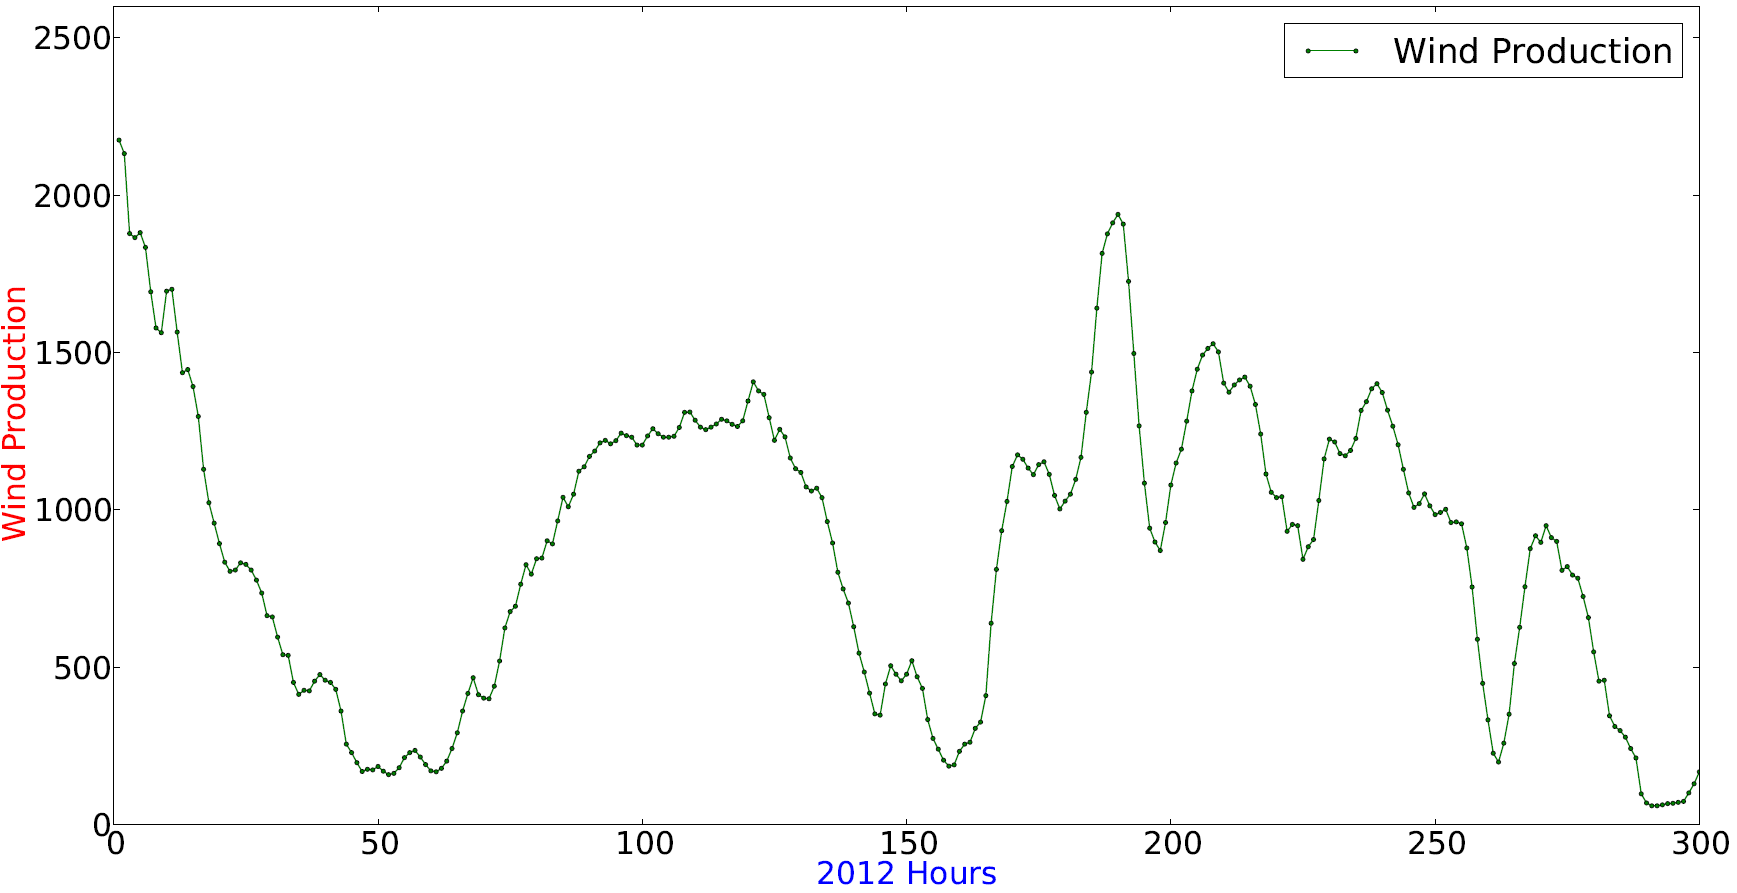
\includegraphics[width=0.99\linewidth,natwidth=898,natheight=587]{billeder/productionTendency400Hours.png}
\caption{Wind production development for 400 hours in 2011}
\label{fig:windHourDevelopment400Hours}
\end{figure}


TEGNING MULTIPE STEP

TALK ABOUT MULTIPLE-STEP-AHEAD FORECASTING --> see karlbranting